\section{Overview}
Producing a dataset suitable for analysis involves the workflow specified in \ref{analysis-workflow}. Effectively this is a 3 stage process, where a user configures and runs the \textit{\_nETL} application to load the data into CouchDB, and then configures a couchDB design document to produce an index and retrieve that index as a CSV. Once a CSV of the joined data has been obtained, it's easy to load the data into Excel and produce a result.

\begin{figure}[ht]
    \centering
    \begin{mdframed}
        \centering
        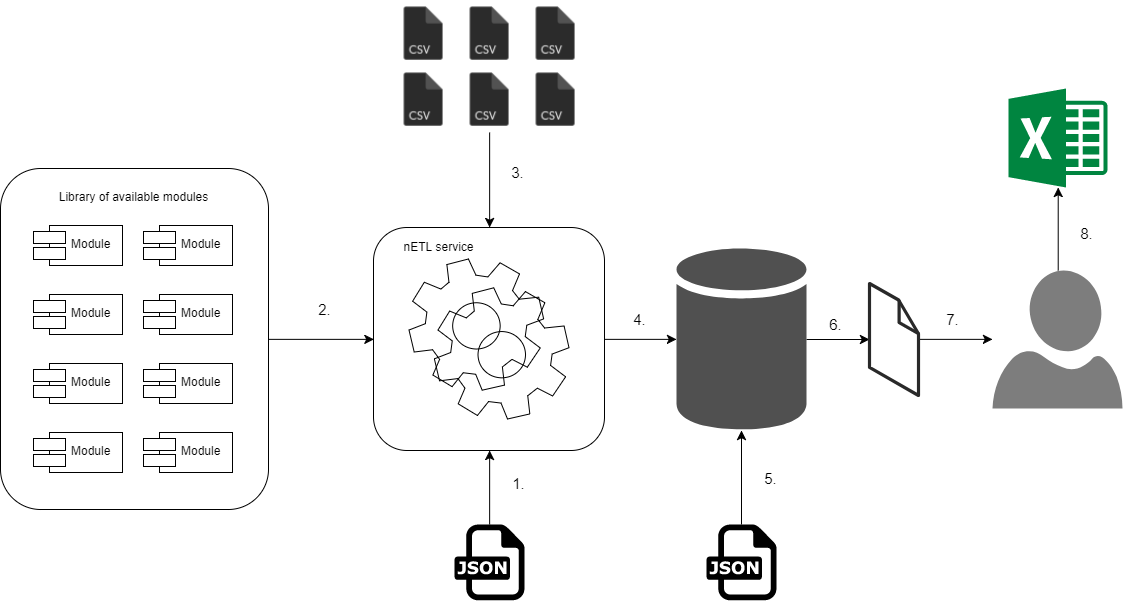
\includegraphics[scale=0.35]{./resources/figures/analysis-workflow.png}
    \end{mdframed}
    \caption[Analysis Workflow]{\textbf{Figure \ref{analysis-workflow}: Workflow to perform an analysis.}1) User creates a configuration file (JSON) that is loaded into the running \textit{\_nETL} service. This configuration includes instructions on which CSVs to load, which modules should be loaded to process the CSVs, and configurations for the modules. 2) Modules are loaded from a library of available modules into the \textit{\_nETL} service. 3) CSVs are loaded into the service, and transformations are applied to the CSV data as specified by the configuration in (1). 4) Data from the CSVs is loaded into CouchDB; this is also achieved via a module specified in (1). 5) A user creates a CouchDB design document, specifying the MapReduce functions, and a List function. 6) The user asks CouchDB to produce the view index as specified by the design document in (5). 7) The user retrieves the data from the view index using the list function specified in (5). 8) The user then loads the resultant CSV into Excel to produce useful metrics.}
    \label{analysis-workflow}
\end{figure}



Joining across the 3 entities (Demographics, Grades and Events), in adherence with the \textit{\_stats} function contract, requires emitting common keys in the map function on which grouping can be performed. To maintain the resolution that exists within the Grade data, that is; \textit{results of a particular student in a particular year for a particular course}, a compound key of the tuple \textless studentID, courseCode, year \textgreater is used for grouping, i.e. for every document processed by the map function, a key:value pair with a key in the form of that tuple needs to be emitted. Emitting this compound key is straightforward for grade data since each document of \textit{type\_} courseGrade has fields for all three of these values. However, neither the demographic nor the event data contains fields for 'courseCode', and student benchmarking in the demographic data are only for the year that student first registered. As such, of the required fields to output the key for joining, Demographic data only contains a 'studentID' field. Documents of \textit{type\_} 'sakaiEvent' include fields for studentId and year, but not courseCode (there is a FK field \textit{course\_id}) but it doesn't point to any field in the grade data.

To produce a key of the tuple \textless studentID, courseCode, year \textgreater for demographic data, the courseCode and year value have to be fabricated. In other words, demographic data has to be duplicated for every possible key combination on which it could be joined. In this case a single demographic document needs to be output for every course that a student can take, and then further duplicated for every year in which a student could take that course. Likewise the event data, which has fields for studentID and year, needs to be duplicated for every course that a student can take. Such an approach to joining is the basis of this analysis, which is done in iterations. Each iteration increases the volume of data processed by the map function so as to get insight in the effectiveness of this approach to joining documents. Analyses are discussed in terms of the results of each iteration. In general, each analysis involves 4 phases of data-wrangling:



Configurations used for \textit{nETL} for all the runs done while creating the analysis described below are shown in the appendix - see \ref{netl-run1-config}). Runtime results of \textit{nETL}, CouchDB indexing times, database/index storage footprints are shown in Table \ref{performance-analysis}. Initial CouchDB view calculation was performed on a local machine, but subsequently to achieving the analysis results, indexing time was compared on different cluster sizes. These times are shown in \ref{couch-indexing}. As seen in the table, increasing the cluster size reduces the time taken to index a database as per the described \textit{MapReduce} function decreases. This is as expected since dispersing documents across shards should be random enough that documents get distributed across shards uniformly (see \ref{slack-7-nov}), meaning that increasing nodes in a cluster reduces the amount of work a node must do when calculating \textit{map} output. However, it is likely that small data sets would not benefit from clustering since there is a high network overhead of sharded databases.

\section{Join of Grades/Demographics}
Creating datasets comprising grade and FU data involved filtering CSVs and loading that data into CouchDB using \textit{nETL}

For a join on the Grades and Demographics entities, the map function is configured to output key-value pairs of the form: \textless studentID, courseCode, year \textgreater : <9 element list>. A description of the 11-element value list is shown in \ref{grades-join-demographics-output}. Configuration for the \textit{nETL} task is shown in the appendix (see \ref{netl-config-grades-join-demographics}), as is the Map function and list function (see\ref{msc-design-doc}).

The list shown in \ref{grades-join-demographics-output} shows ALL the values output by a map function on the join between all three entities. For the first two runs, event information is NOT emitted.

\begin{figure}[ht]
    \centering
    \begin{minted}{javascript}
 [
    // Grade Entitty output
    "CSC1015F %",

    // Demographic Entity output
    "Gr12 Eng %", 
    "Gr12 Sci %",
    "Gr12 Mth %",
    "Gr12 Mth Lit %",
    "Gr12 Mth Adv %",
    "NBT AL %",
    "NBT QL %",
    "NBT Mth %",

    // Event entity output
    "eventCount S1", // Only included for Run 3/4
    "eventCount S2" // Only included for Run 3/4
 ]    
    \end{minted}
    \caption[2-way-join map output]{\textbf{Figure \ref{grades-join-demographics-output}: Output of map function for grades joined with demographics.} This list, shown as a JavaScript array, is the key to the map function output. In other words, the map function outputs a list of values that correspond to this list. When retrieving the view output, headers can be given back to the columns retrieved using this key. View output can be achieved via a List function (as has been done in this project), or via bespoke JavaScript code.}
    \label{grades-join-demographics-output}
\end{figure}

% Runs
\subsection{CS1015F: Course grades vs Student Benchmarks}


across the FU data and course grades for CSC1015F,


To create the dataset to show correlation between student benchmarking and achieved grades in the CS1015F course for undergraduates, \textit{nETL} was configured to filter Grade data on the field 'Course' to only allow the value 'CS1015F' in addition to the filtering and transforming \textit{nETL} is configured to on all Grade rows as described in the data overview. Additional filtering on the Demographic entity is performed on the StudentID field (anonIdnew) to load demographic data of the students who took the CSC2015F course. This list of students was prepared by Excel filtering, but could just as easily have been performed in CouchDB or any other database if the size of the file did not allow for opening in Excel. Since the view index is small, the list function returns the CSV output instantly. The CSV output size is 67Kb

\subsection{Run 2: Multiple Courses}
With the ease at which the \textit{nETL} software handled loading data in Run 1, and the ease at which CouchDB was able to handle indexing, a second run was created with multiple courses. For this run, 40 courses were selected: ECO1010F, ECO1011S, ACC1006F, STA1000S, ECO2003F, BUS1036F, ECO2004S, CML1001F, MAM1010F, PSY1004F, FTX2024S, ECO2007S, ACC2011S, CSC1015F, PHI2043S, ACC3023S, INF2004F, PSY1005S, STA2020F, CML2010S, CML2001F, SOC1001F, ACC2018S, SOC1005S, BUS2010F, ACC2012W, AXL1100S, ACC3022H, ACC3004H, PHY1012F, MAM1020F, PHI2043F, FTX3045S, ACC3009W, MAM1012S, FTX3044F, MAM1000W, POL1004F, CSC1016S, ACC4000H. These courses were selected simply because they have a high level of student enrollment. \textit{nETL} filtering on the courseCode field was configured to allow all these codes. Filtering on student IDs in the demographic was removed, since over 10 000 student numbers would need to be included a list for such a filter.

Compared to Run1, there is a significant increase in the size footprint of the view index (from \textless 1MB to 143MB) do to the requirement of duplicating demographic output in the map function. Performance of the list function degraded considerably, with streaming of the 2MB CSV taking several minutes. To efficiently retrieve view output of larger indexes would require implementing data retrieval outside of CouchDB. List functions require iterating through every view output individually, whereas working with the view directly would allow for retrieving in batches which is much more efficient. \textit{nETL} could be configured to do this, but hasn't been.

\subsection{Correlation analysis}
The results for \textit{Run 1} and \textit{Run 2} have been summarized in the graphs in Figure \ref{run1-chart1}; several courses were picked at random to show correlation between course grades and student benchmarks. The results show that in general, higher benchmarking scores are indicative of higher course results overall. Some of the benchmarks show stronger correlation to grade results than other, as seen by steeper trendline gradient.

\begin{figure}[H]
    \centering
    \begin{mdframed}
        \centering
        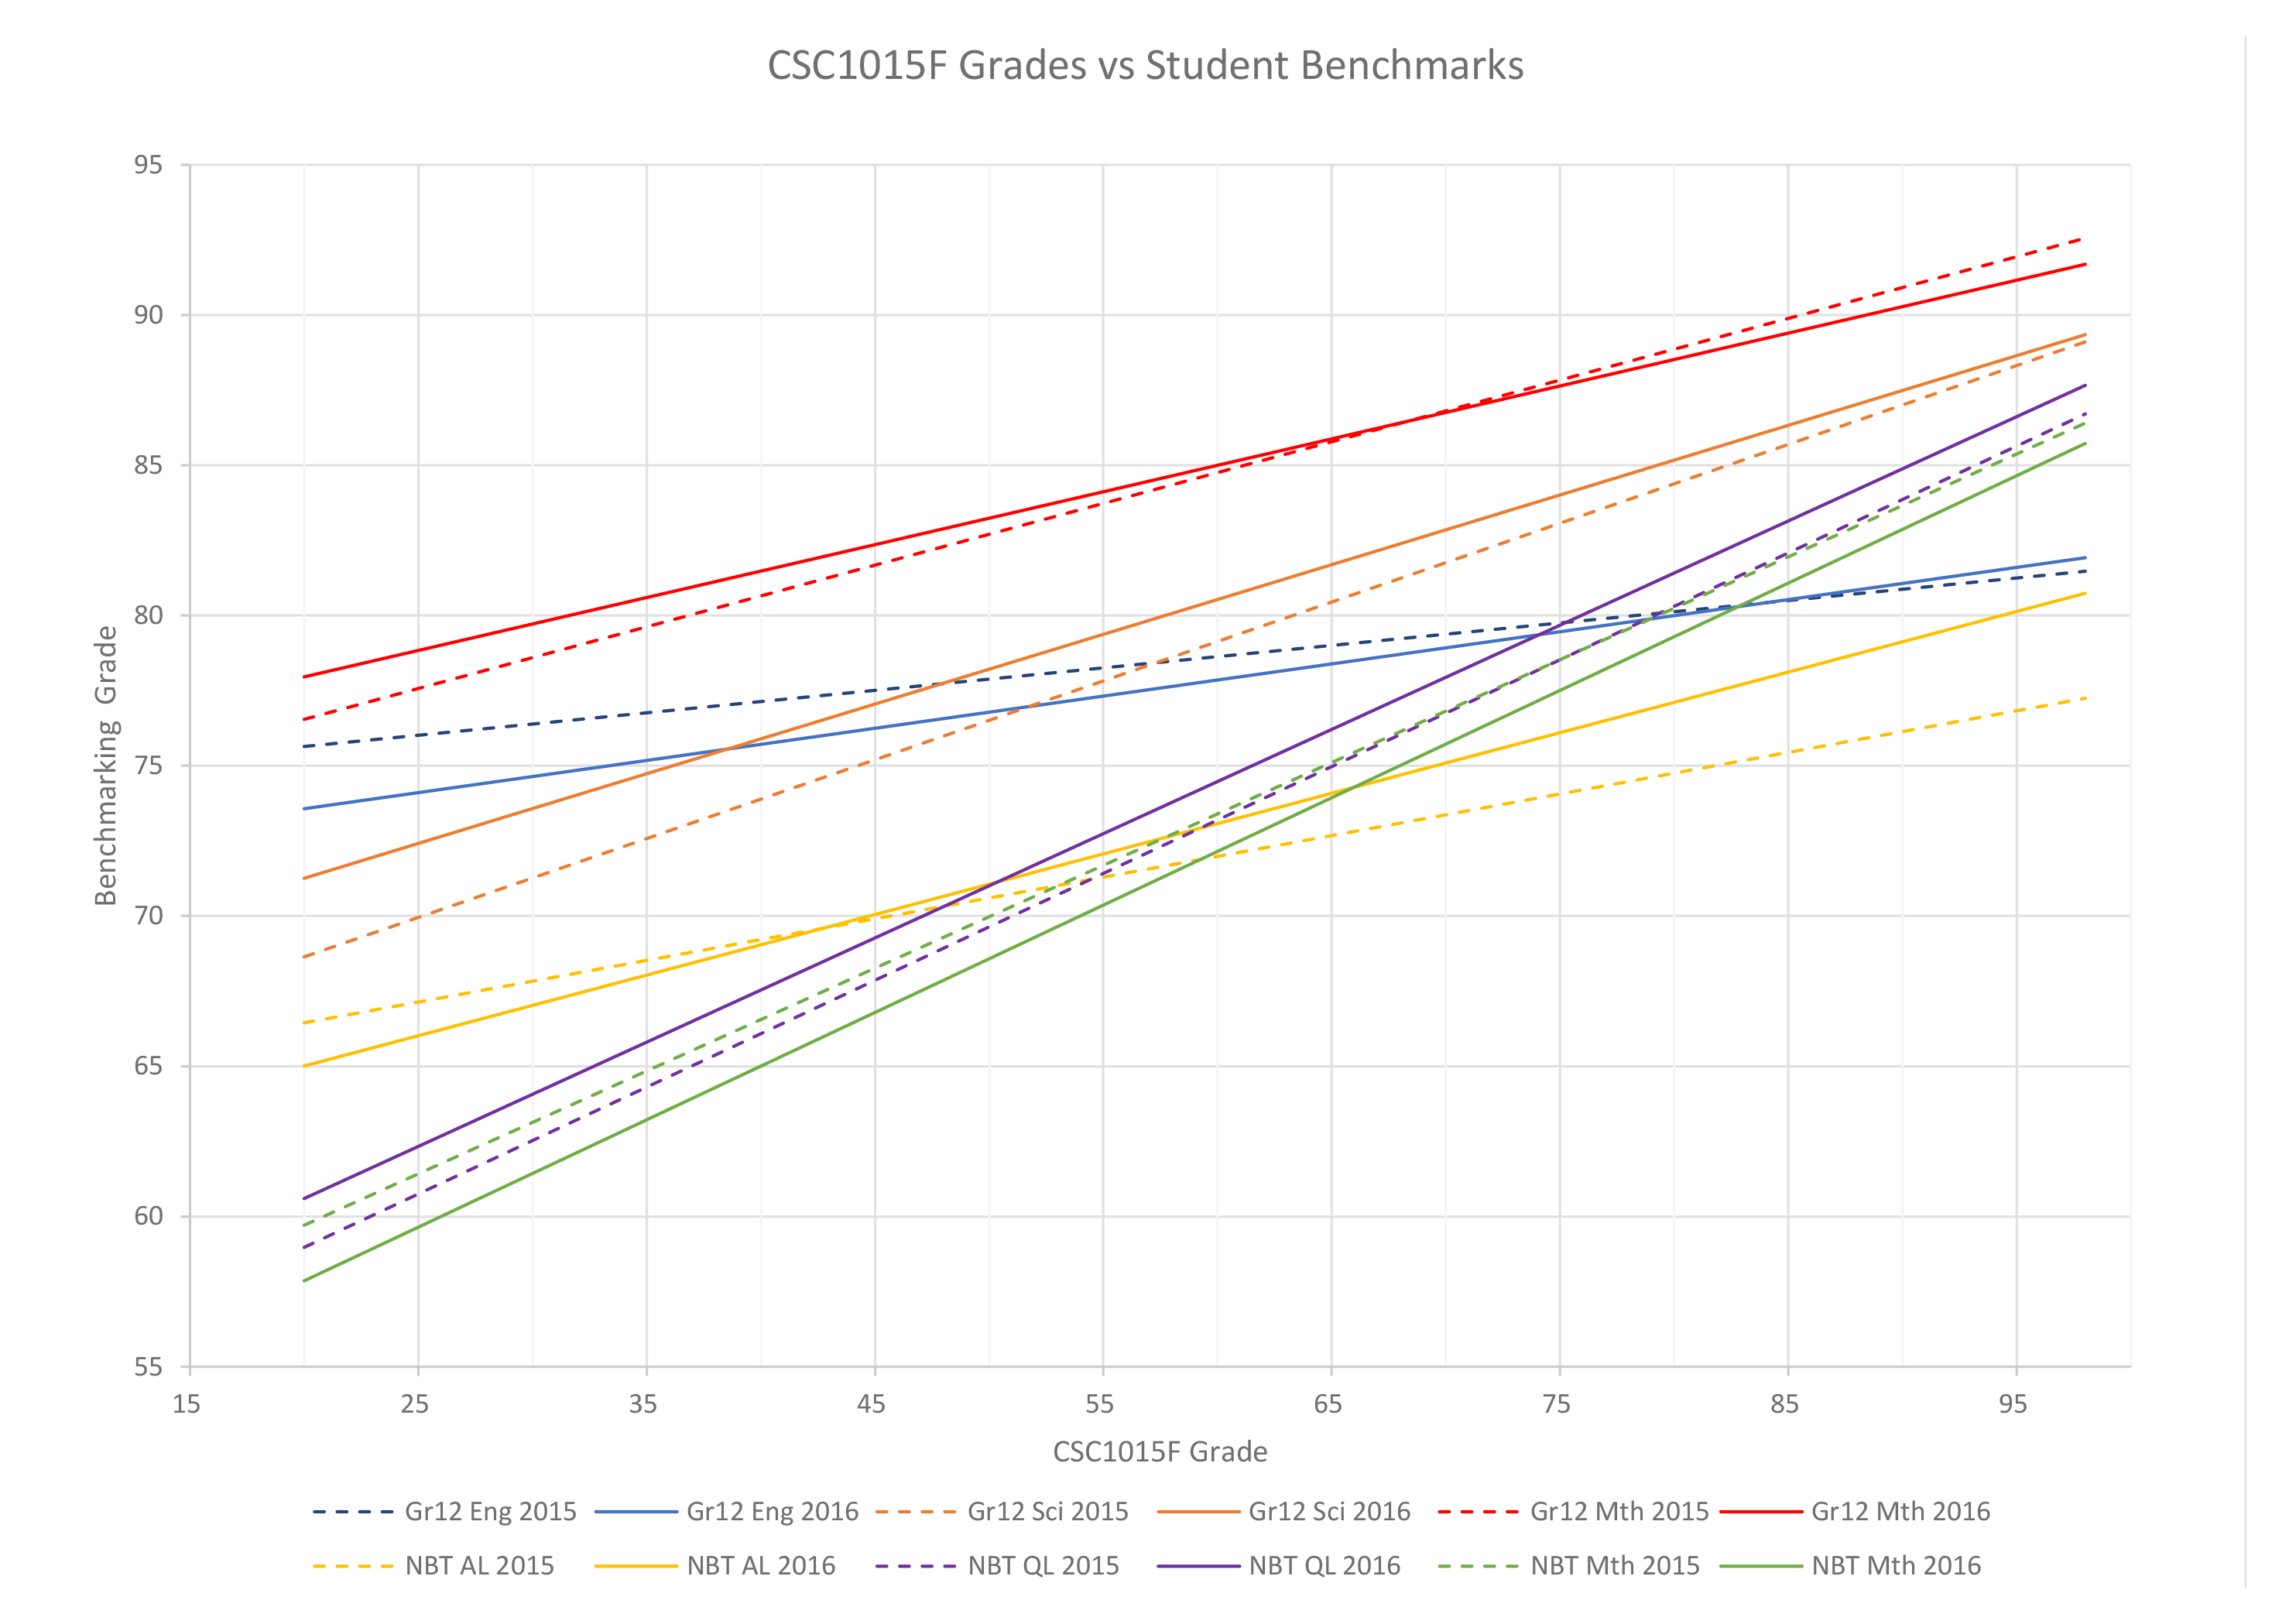
\includegraphics[scale=0.55]{./resources/figures/run1-chart1.png}
    \end{mdframed}
    \caption[CSC1015 grade vs benchmark correlation]{\textbf{Figure \ref{run1-chart1}: Correlation between student benchmarks and CSC1015F results.} This graph shows benchmark scores plotted against the final CSC1015F grade. Datasets focus on a single benchmark, so a trendline shows the correlation between a single benchmark and final grades.}
    \label{run1-chart1}
\end{figure}

\section{join of Grades/Demographics/Events}

% Runs
\subsubsection{Run 3: CS1015F}
Building on the results from \textit{Run 1}, a join on events data was added. To achieve this, n\textit{nETL} was reconfigured to filter grades for only 2016 (since event data is only available for 2016), and an additional \textit{nETL} task was configured to load event data. Filtering on the event data was performed on the (anonymized) uct\_id field to include only events from students who took the CSC1015F course in 2016. This list was derived from the Grade data using Excel.


\subsubsection{Run 4: Multiple Courses}


\subsubsection{Correlation analysis}
